\documentclass[12pt]{article}
\usepackage{fullpage}
\usepackage{graphicx}
\usepackage{sidecap}
\usepackage{algorithmic}
\usepackage{algorithm2e}
\usepackage{bbm}
\usepackage{amssymb}
\usepackage{amsmath}
\usepackage{amsfonts}
\usepackage{amsthm}
\usepackage{yhmath}
\usepackage{siunitx}
\usepackage[mathscr]{euscript}
\usepackage{enumerate}
\usepackage{mathtools}
\usepackage[hmargin=1in,vmargin=1in]{geometry}
\usepackage{graphicx}
\usepackage{subfigure}
\usepackage{setspace}
\usepackage{systeme}
\linespread{1.4142}
\graphicspath{ {./images/} }


\title{GAMES ON POKER STREET}
\date{December 5, 2024}
\begin{document}
\maketitle

\begin{abstract}

In this paper we present strategies that are fundamentally sound; that is, yield no benefit to an opponent's attempt to exploit us. The games presented contain the following elements: there are at least two or more players, at least one player has a choice of action(s), the game has a set of outcomes for each player, and the outcomes depend on the choices of actions by the players. While the models presented are simplified toy games and do not fully represent poker, they provide key pieces of the strategic puzzle. By examining various game variations, we will highlight the strategic thinking players can apply to make optimal decisions in different scenarios.

\end{abstract}

\section{Definitions}

\textbf{Definition 2.1}: \textbf{(Poker) street} is a round of betting and cards turned in a game of poker, consisting of four in total: pre-flop, flop, turn, and river.
\\
\textbf{Definition 2.2}: \textbf{Half - street game} consists of two players. First player, X, checks. The second player, Y, has the option to check or bet some amount. If Y bets, X then can fold or call.
\\
\textbf{Definition 2.3}: \textbf{Showdown} is when both players show their hands and determine winner. 
\\
\textbf{Definition 2.4}: \textbf{Value} is the expectation for Y assuming both sides play optimally.
\\
\textbf{Definition 2.5}: \textbf{Ex-showdown} is the value played in particular half-street game.
\pagebreak
\section{Clairvoyance game}

\textbf{Game Setup}
\begin{itemize}
    \item One half-street
    \item Pot size of $P$ bets
    \item Limit betting
    \item $Y$ is clairvoyant, meaning they know X's hand.
\end{itemize}

\noindent\textbf{Modeling the Game:}  
Each player has one card. Without loss of generality, let $X$ have card $S$.  
$Y$ chooses randomly 1 card from a pile of $n$ cards where $\frac{n}{2}$ cards have a value beating $S$ and $\frac{n}{2}$ have a value losing to $S$.

Since $Y$ can see both their card and $X$'s card, $Y$ knows immediately if they have:
\begin{itemize}
    \item \textbf{Nuts} (winning hand)
    \item \textbf{Dead hand} (losing hand)
\end{itemize}

\noindent Thus, we can create two payoff tables to model this scenario:
\begin{enumerate}
    \item Table 1 corresponds to $Y$ having \textbf{nuts}.
    \item Table 2 corresponds to $Y$ having a \textbf{dead hand}.
\end{enumerate}

\subsection*{Payoff Tables}

\paragraph{Table 1 ($Y$ has nuts):}
Payoffs are shown in terms of $Y$.

\[
\begin{array}{|c|c|c|}
\hline
 & \text{Check-Call (X)} & \text{Check-Fold (X)} \\
\hline
\text{Bet (Y)} & +1 & 0 \\
\hline
\text{Check (Y)} & 0 & 0 \\
\hline
\end{array}
\]

\paragraph{Table 2 (Y has dead hand):}
Payoffs are shown in terms of $Y$.

\[
\begin{array}{|c|c|c|}
\hline
 & \text{Check-Call (X)} & \text{Check-Fold (X)} \\
\hline
\text{Bet (Y)} & -1 & +P \\
\hline
\text{Check (Y)} & 0 & 0 \\
\hline
\end{array}
\]

\subsection*{Analysis}
\begin{itemize}
    \item \textbf{Dominated Strategy in Table 1:} Under ideal play, $Y$ will never check when they have the nuts, as betting always results in an equal or higher payoff. Thus, $Y$ has a pure strategy of always Betting.

    \item \textbf{Dominated Strategy in Table 2:} Under ideal play, $X$ will never fold when $Y$ has a dead hand. The only problem is that since only $Y$ is clairvoyant, $X$ doesn't know if $Y$ has the nuts or a dead hand. 

    \item \textbf{Pattern of Responses:} \vspace{3mm}\\ 
    Tables 1 and 2 can be seen as one table for the view of \(X\). From this, we can see the cyclical nature of best response:  
    \begin{itemize}
        \item \(Y\) should initially bet on all nuts and check all dead hands; this causes \(X\) to fold all hands.
        \item Then \(Y\) will bet all hands; causing \(X\) to call all hands.
        \item Finally, \(Y\) will revert back to their original strategy.
    \end{itemize}

    \item \textbf{Balanced Strategy: Indifference Between Betting and Bluffing} \vspace{3mm}\\
    In a balanced strategy between betting and bluffing, the expected value of making a value bet (where you actually have a strong hand) should be the same as the expected value of bluffing (where you do not have a strong hand but want to represent one). Y's goal is to create a situation where X is indifferent between calling and folding in response to your bet.
    
    Thus, the equation is:  
    \[
    \text{Pot size} \cdot \text{FreqXFolds} = \text{Bluff bet} \cdot \text{FreqXCalls}
    \]
    \[
    \text{P(1~-~C) = C} \implies C = \frac{P}{P+1}
    \]
    
    where the left-hand side is the expected value for \(Y\) when \(X\) folds is the pot size, which occurs with probability FreqXFolds.

    And the Right-hand side is the expected value for \(Y\) when \(X\) calls the bluff. If \(Y\) has the nuts, \(Y\) wins the pot; however, if \(Y\) has a dead hand, \(Y\) loses the bluff bet. Therefore, the expected outcome for \(Y\) is scaled by FreqXCalls.

    \textbf{Notice}, as the pot size increases, the rate of \(X\) calling increases. As there is more money at stake, \(X\) is less willing to give it up. Additionally, \(X\) must call more to keep \(Y\) from bluffing.

\item \textbf{Finding $b$, $Y$'s ideal bluff-to-bet ratio}

To find \(\beta\), \(Y\)'s ratio of how often they should bluff vs bet, we can set the outcomes from responses of \(X\) equal to each other. If \(X\) calls, they lose 1 bet by calling a value bet and gain \(P + 1\) by calling a bluff.  
\[
1 = (P + 1)\beta \implies \beta = \frac{1}{P+1}
\]
Note, \(X\) must call enough to make \(Y\) indifferent to betting and checking. From earlier:  
\[
C = \frac{P}{P+1} = (1-\beta), \quad \text{where } C \text{ is the frequency of } X \text{ calling.}
\]

\item \textbf{Ratio \(1-\beta\):}  
\[
1 - \beta = 1 - \frac{1}{P+1}.
\]
\[
1 - \beta = \frac{P}{P+1}.
\]
Generalization to games with variable bet sizes (\(s\)):  
\[
\beta = \frac{s}{1+s} \quad\text{, where } s \text{ is the bet size in pots.}
\]
Note, as the pot size increases, \(s\) decreases, and so does \(\beta\). Thus, \(Y\) bluffs less into larger pots.

\item \textbf{Optimal Strategies:}
\begin{itemize}
    \item \(Y\) bets all their nut hands and bluffs $\beta$ of their dead hands, or \(\beta/2\) of their total hands.
    \item \(X\) calls with \(1 - \beta\) of their hands total.
\end{itemize}
    Note, by itself, bluffing is not a profitable play over time. A combination of both bluffing and value betting is needed to ensure optimal strategy gains, assuming your opponent is playing optimally.
    
\item \textbf{Expected Value of Y:}
    \begin{align*}
        \langle Y \rangle &= 0.5 \cdot \langle Y \rangle (\text{when Y has Nuts}) + 0.5 \cdot \langle Y \rangle (\text{when Y has Dead hand}) \\
        \langle Y \rangle &= 0.5 \cdot [C \cdot 1 + (1-C)\cdot 0] + 0.5 \cdot [C\cdot(-1) + (1-C)\cdot P] \\
        &= 0.5 \cdot C + 0.5 \cdot [-C + P - C \cdot P] \\
        &= 0.5 \cdot P - 0.5 \cdot C \cdot P \\
        &= 0.5 \cdot P - 0.5 \cdot \left[\frac{P}{P+1}\right] \cdot P \\
        &= 0.5 \cdot P \cdot \left[1 - \frac{P}{P+1}\right] \\
        &= 0.5 \cdot P \cdot \frac{1}{P+1} \\
        \langle Y \rangle &= \frac{P}{2(P+1)}
    \end{align*}

\item \textbf{Sensitivity Analysis of Pot Size (\(P\)) on Key Variables:}
\[
\begin{array}{|c|c|c|c|}
\hline
P \, \text{(Pot Size)} & \beta = \frac{1}{P+1} & C = \frac{P}{P+1} & \langle Y \rangle = \frac{P}{2(P+1)} \\
\hline
1 & 0.5 & 0.5 & 0.25 \\
5 & 0.167 & 0.833 & 0.417 \\
10 & 0.091 & 0.909 & 0.455 \\
50 & 0.019 & 0.981 & 0.490 \\
100 & 0.010 & 0.990 & 0.495 \\
1000 & 0.001 & 0.999 & 0.499 \\
10^6 & 10^{-6} & 1.000 & 0.500 \\
\hline
\end{array}
\]

\textbf{Notice:}
\begin{itemize}
    \item As \(P\) increases, $\beta$, $Y$'s bluff to bet ratio, decreases $$\lim_{P \to \infty} \beta = 0$$
    \item As \(P\) increases, so does \(C\), the frequency of $X$ calling \[\lim_{P \to \infty} C = 1\]
    \item As \(P\) increases, so does \(Y\)'s expected value (\(\text{EV}\)) \[\lim_{P \to \infty} \langle Y \rangle = 0.5\]
\end{itemize}

So far, we have made made the assumption that $Y$ chooses randomly 1 card from a pile of $n$ cards where $\frac{n}{2}$ cards have a value beating $S$ and $\frac{n}{2}$ have a value losing to $S$.

What if this is not the case? 

Let $\alpha$ denote the probability that $Y$ has nuts and $1-\alpha$ denote the probability that $Y$ has a dead hand.

\item \textbf{General Formula for Expected Value of $Y$:}
    \begin{align*}
        \langle Y \rangle &= \alpha \cdot \langle Y \rangle (\text{when $Y$ has Nuts}) + (1-\alpha) \cdot \langle Y \rangle (\text{when $Y$ has Dead hand}) \\
        \langle Y \rangle &= \alpha \cdot [C \cdot 1 + (1-C)\cdot 0] + (1-\alpha) \cdot [C\cdot(-1) + (1-C)\cdot P] \\
        &= \alpha C + (1-\alpha) \cdot [-C + P - CP] \\
        &= \alpha C - C(1-\alpha) + P(1-\alpha) - CP(1-\alpha)\\
        &= 2\alpha C - C + P - \alpha P - CP + \alpha CP\\
        &= C \cdot (2\alpha - 1 - P + \alpha P) + P - \alpha P\\
        &= \frac{P}{P+1} \cdot (2\alpha - 1- P + \alpha P) + P - \alpha P \\
        &= \frac{P \cdot (2\alpha - 1 - P + \alpha P) + (P + 1)(P - \alpha P)}{P + 1} \\
        &= \frac{2\alpha P - P - P^2 + \alpha P^2 + P^2 - \alpha P^2 + P - \alpha P}{P + 1} \\
        \langle Y \rangle &= \frac{\alpha P}{P+1}
    \end{align*}

\end{itemize}

\section{[0,1] game}

\hspace{\parindent} This section introduces the concept of betting and calling region, similar to the previous section, but in non-clairvoyant setting.

\textbf{Game Setup}
\begin{itemize}
    \item One half-street
    \item Each player get a number in [0,1]
    \item Player with lower number wins.
\end{itemize}

\subsection{Game \#1}

\textbf{Rules:} the first player can only check or call to second player's bet.

\hspace{\parindent}In this game, the only player to make a move is the second player. Then there exists a threshold, $y_0 \in \left[0,1\right]$, such that the second player will fold if their hand is above that number, and will bet otherwise. 

Consider $y_0$. The probability of the first player get a number less than $y_0$, or the first player wins, is exactly $y_0$. By extension, the probability of the second player wins is $1-y_0$. 

Then the expected value of the second player is $1\times y_0 + (-1) \times(1-y_0)$. Since the second player is the only one to make a move, they will want to maximize their expected value, or at least making it positive. Thus $1\times y_0 + (-1)\times(1-y_0) \ge 0$, so $y_0 \ge 0.5$. So the optimal play for second player is to bet half of the time.

\begin{center}
\begin{tabular}{|c | c|} 
 \hline
 \textbf{X's hand} & \textbf{Y's Result} \\ [0.5ex] 
 \hline
 [0,$y_0$] & -1 (X calls with better hand)  \\ 
 \hline
 [$y_0$,1] & 1 (X calls with worse hand)\\
    \hline
\end{tabular}
\end{center}

\subsection{Game \#2}

\textbf{Rules:} the first player can now fold or call to second player's bet.

Suppose that the second player plays the same strategies as in Game \#1. Then, for the first player, there exists a threshold, $x_0$, such that they will call Y's bet when X gets a number lower than $x_0$, and fold otherwise. 

Suppose that X calls bet on $x_0$. Then they will lose if Y's number is lower than $x_0$, and they will win if Y's number is between $x_0$ and $y_0$. 

Let $P$ be the pot value after X checks in the first turn. After Y's bet, the pot value is $P+1$. If X wins, the reward is $P+1$. If X bets and lose, the loss is $1$, the value of the bet. 

So, the expected value for X is $(P+1)\cdot(y_0-x_0) + (-1) \cdot (x_0)$. Since X will try to play optimally, this expected value is positive. The solution for $x_0$ yields $x_0 < y_0\times \frac{P+1}{P+2}$. In addition, we get $x_0 < y_0$.

The full game follows:
\begin{center}
\begin{tabular}{|c|c|c|}
    \hline
     X's hand & Y's hand & Result \\
     \hline
     $[0,x_0]$ & $[0,x_0]$ & Draw\\
     \hline
     $-$& $[x_0, y_0]$ & X wins +1\\
    \hline
     $-$& $[y_0, 1]$ & n/a \\
    \hline
     $[x_0, y_0]$& $[0, x_0]$ & Y wins pot\\
    \hline
     $-$& $[x_0, y_0]$ & Y wins pot\\
    \hline
     $-$& $[y_0, 1]$ & n/a\\
    \hline
     $[y_0, 1]$& $[0, x_0]$ & Y wins pot\\
    \hline
     $-$& $[x_0, y_0]$ & Y wins pot\\
    \hline
     $-$& $[y_0, x1]$ & Draw\\
    \hline
\end{tabular}
\end{center}
From the table, since X is much more likely to fold to Y's bet, Y is more likely to win. In the final row, the game is draw due to Y's checking and X's folding. Here, Y can improve their chance by bluffing, or placing a bet despite a bad hand. If the new threshold is $y_1 > y_0$, the last row will become: 

\begin{center}
    \begin{tabular}{|c|c|c|}
        \hline
        X's hand & Y's hand & Result \\
        \hline
         $[y_0, 1]$& $[y_0, y_1]$ & Draw \\
         \hline
         $-$ & $[y_1, 1]$ & Y wins pot \\
         \hline \end{tabular}
\end{center}

Since Y can unilaterally improve their expected value, this is not an optimal play for X. This game illustrates the concept of betting and checking region, and it shows that how bluffing can be advantageous.

\section{AKQ game}

\subsection*{Version 1}
\begin{itemize}
    \item One half-street.
    \item Pot size of 2 units (initial ante-in).
    \item Limit betting of 1 unit.
\end{itemize}

\noindent\textbf{Modeling the Game:}  
After the ante, each player is dealt one card without replacement from a deck of 1 Ace ($A$), King ($K$), and Queen ($Q$). $A$ beats $K$, and $K$ beats $Q$.

Both players ante and are then dealt their cards. $Y$ acts first and can bet or check. $X$ may respond by calling or folding. Based on this, we construct the following matrices.

\begin{itemize}
    \item \textbf{Ex-showdown payoff matrix for Y:}
    \[
    \begin{array}{|c|c|cc|cc|cc|}
    \hline
    & Y & \text{Ace} &  & \text{King} &  & \text{Queen} & \\
    \hline
    X & & \text{Bet} & \text{Check} & \text{Bet} & \text{Check} & \text{Bet} & \text{Check} \\
    \hline
    \text{Ace} & \text{Call} & - & - & -1 & 0 & -1 & 0 \\
    & \text{Fold} & - & - & +2 & 0 & +2 & 0 \\
    \hline
    \text{King} & \text{Call} & +1 & 0 & - & - & -1 & 0 \\
    & \text{Fold} & +0 & 0 & - & - & +2 & 0 \\
    \hline
    \text{Queen} & \text{Call} & +1 & 0 & +1 & 0 & - & - \\
    & \text{Fold} & 0 & 0 & 0 & 0 & - & - \\
    \hline
    \end{array}
    \]

    \item Notice that we can iteratively remove dominated strategies.
    
    \item \textbf{Simplified matrix:}
    \[
    \begin{array}{|c|c|c|cc|}
    \hline
         & Y & \text{Ace} & \text{Queen} &\\
    \hline
       X  & & \text{Bet} & \text{Bet} & \text{Check} \\
    \hline
       \text{Ace} & \text{Call} & - & -1 & 0 \\
    \hline
        \text{King} & \text{Call} & +1 & -1 & 0 \\
        & \text{Fold} & 0 & +2 & 0 \\
    \hline
    \end{array}
    \]

    \item \textbf{Oscillating pure strategies:}
    \begin{itemize}
        \item If $X$ always calls with $K$, $Y$ only value bets.
        \item If $X$ always folds with $K$, $Y$ bluffs all $Q$.
        \item Cycles back: $X$ always calls with $K$.
    \end{itemize}

    \item \textbf{Key strategies:}
    \begin{itemize}
        \item At what frequency should $X$ call with $K$?
        \item At what frequency should $Y$ bluff with $Q$?
    \end{itemize}
\end{itemize}

\noindent\textbf{Expected Payoff Analysis:}
\begin{itemize}
    \item \(Y_1\) $Y(Q)$: always bluff
    \item \(Y_2\)$ Y(Q)$: always check
    \item \(X_1\) $X(K)$: always calls
    \item \(X_2\) $X(K)$: always folds
\end{itemize}


\begin{itemize}
    \item \(\langle Y_1, X_1 \rangle\):  
    \[
    \begin{aligned}
    [Y(A)|X(K)] &= +1 \cdot \frac{1}{6} = \frac{1}{6}, \\
    [Y(A)|X(Q)] &= +0 \cdot \frac{1}{6} = 0, \\
    Y(K) &= +0 \cdot \frac{1}{3} = 0, \\
    Y(Q) &= -1 \cdot \frac{1}{3} = -\frac{1}{3}.
    \end{aligned}
    \]
    Total: \(\langle Y_1, X_1 \rangle = -\frac{1}{6}\).

    \item \(\langle Y_2, X_1 \rangle\):  
    \[
    \begin{aligned}
    [Y(A)|X(K)] &= +1 \cdot \frac{1}{6} = \frac{1}{6}, \\
    [Y(A)|X(Q)] &= +0 \cdot \frac{1}{6} = 0, \\
    Y(K) &= +0 \cdot \frac{1}{3} = 0, \\
    Y(Q) &= +0 \cdot \frac{1}{3} = 0.
    \end{aligned}
    \]
    Total: \(\langle Y_2, X_1 \rangle = +\frac{1}{6}\).
    
    \item \(\langle Y_1, X_2 \rangle\):  
    \[
    \begin{aligned}
    Y(A) &= +0 \cdot \frac{1}{3} = 0, \\
    Y(K) &= +0 \cdot \frac{1}{3} = 0, \\
    [Y(Q)|X(K)] &= +2 \cdot \frac{1}{6} = +\frac{2}{6}, \\
    [Y(Q)|X(A)] &= -1 \cdot \frac{1}{6} = -\frac{1}{6}.
    \end{aligned}
    \]
    Total: \(\langle Y_1, X_2 \rangle = +\frac{1}{6}\).

    \item \(\langle Y_2, X_2 \rangle\):  
    \[
    \begin{aligned}
    Y(A) &= +0 \cdot \frac{1}{3} = 0, \\
    Y(K) &= +0 \cdot \frac{1}{3} = 0, \\
    Y(Q) &= +0 \cdot \frac{1}{3} = 0.
    \end{aligned}
    \]
    Total: \(\langle Y_2, X_2 \rangle = +0\).
\end{itemize}

\begin{table}[h]
    \centering
    \begin{tabular}{|l|c|c|}
        \hline
        & \(Y_1\) - bets queens & \(Y_2\) - checks queens \\ \hline
        \(X_1\) - calls with kings & +1 & -1 \\ \hline
        \(X_2\) - folds with kings & -1 & 0 \\ \hline
    \end{tabular}
    \caption{Payoff Matrix for Mixed Strategies}
    \label{tab:payoff_matrix}
\end{table}

\noindent\textbf{Final Analysis:}  
Both X and Y will adopt mixed strategies:
\begin{itemize}
    \item X calls with K $\frac{1}{3}$ of the time.
    \item Y bluffs with Q $\frac{1}{3}$ of the time.
\end{itemize}

\noindent This aligns with the solution derived from the Clairvoyance game where \(\alpha = \frac{1}{P+1}\). Since the pot size is 2 in AKQ, we find \(\alpha = \frac{1}{3}\).

\textbf{Value of Game From Y's View:}
\begin{itemize}
    \item Probability of each outcome: \(\frac{1}{6}\)
    \item Outcomes: 
    \[
    P[(A,K) + (A,Q) + (K,A) + (K,Q) + (Q,A) + (Q,K)]
    \]
    \item Calculation:
    \[
    \langle Y \rangle = \frac{1}{6} \bigg[
        \bigg( \frac{2}{3}(0) + \frac{1}{3}(1) \bigg) + 
        (0) + (0) + (0) + 
        \bigg( \frac{2}{3}(0) + \frac{1}{3}(-1) \bigg) + 
        \bigg( \frac{2}{3}(0) + \frac{1}{3} \bigg( \frac{2}{3}(2) + \frac{1}{3}(-1) \bigg) \bigg)
    \bigg]
    \]
    \item Simplification:
    \[
    \langle Y \rangle = \frac{1}{6} \bigg( \frac{1}{3} + \frac{-1}{3} + \frac{1}{3} \bigg)
    \]
    \item Final Value:
    \[
    \langle Y \rangle = \frac{1}{18}
    \]
\end{itemize}

\subsection*{Version 2}
\begin{itemize}
    \item One half-street.
    \item Pot size of \( P \) units.
    \item Limit betting of 1 unit.
\end{itemize}

\begin{itemize}
    \item \textbf{Ex-showdown payoff matrix for \( Y \):}
    \[
    \begin{array}{|c|c|cc|cc|cc|}
    \hline
    & Y & \text{Ace} &  & \text{King} &  & \text{Queen} & \\
    \hline
    X & & \text{Bet} & \text{Check} & \text{Bet} & \text{Check} & \text{Bet} & \text{Check} \\
    \hline
    \text{Ace} & \text{Call} & - & - & -1 & 0 & -1 & 0 \\
    & \text{Fold} & - & - & +P & 0 & +P & 0 \\
    \hline
    \text{King} & \text{Call} & +1 & 0 & - & - & -1 & 0 \\
    & \text{Fold} & 0 & 0 & - & - & +P & 0 \\
    \hline
    \text{Queen} & \text{Call} & +1 & 0 & +1 & 0 & - & - \\
    & \text{Fold} & 0 & 0 & 0 & 0 & - & - \\
    \hline
    \end{array}
    \]

    \item Notice that we can iteratively remove dominated strategies.
    
    \item \textbf{Simplified matrix:}
    \[
    \begin{array}{|c|c|c|c c|}
    \hline
         & Y & \text{Ace} & \text{Queen} &\\
    \hline
       X  & & \text{Bet} & \text{Bet} & \text{Check} \\
    \hline
       \text{Ace} & \text{Call} & - & -1 & 0 \\
    \hline
        \text{King} & \text{Call} & +1 & -1 & 0 \\
        & \text{Fold} & 0 & +P & 0 \\
    \hline
    \end{array}
    \]
\end{itemize}

\noindent\textbf{Expected Value of \( Y \)'s Bluff:}
\begin{align*}
    \langle Y, \text{bluff} \rangle &= \text{(Lose to Aces)} + \text{(Lose to Kings)} + \text{(Kings Fold, Win the Pot)} \\
    &= \left(\frac{1}{2} \cdot (-1)\right) + \left(\frac{1}{2} \cdot c \cdot (-1)\right) + \left(\frac{1}{2} \cdot (1 - c) \cdot P\right) \\
    &= -\frac{1}{2} - \frac{1}{2}c + \frac{1}{2}P - \frac{1}{2}Pc.
\end{align*}

\noindent\textbf{Expected Value of \( Y \)'s Check:}

\[
    \langle Y, \text{check} \rangle = 0.
\]

\noindent\textbf{Solving for \( c \):}

Starting from: $$-\frac{1}{2} - \frac{1}{2}c + \frac{1}{2}P - \frac{1}{2}Pc = 0$$ we simplify: $$\frac{1}{2} + \frac{1}{2}c - \frac{1}{2}P + \frac{1}{2}Pc = 0.$$

Multiply by 2 to eliminate the fractions:
\[
    1 + c - P + Pc = 0.
\]

Rearranging terms:
\[
    (P + 1)c = P - 1.
\]

Solve for \( c \):
\[
    c = \frac{P - 1}{P + 1}.
\]

\noindent\textbf{Expected Value of \( X \)'s Call:}
\begin{align*}
    \langle X, \text{call} \rangle &= \text{(Lose to Aces)} + \text{(Win against Queens)} \\
    &= \frac{1}{2}(-1) + \frac{1}{2}[b(1)] \\
    &= -\frac{1}{2} + \frac{1}{2}b.
\end{align*}

\noindent\textbf{Expected Value of \( X \)'s Fold:}

\[
    \langle X, \text{fold} \rangle = \frac{1}{2}(b)(-P).
\]

\noindent\textbf{Finding the Optimal Calling Frequency:}

To make \( X \) indifferent between calling and folding:
\[
    \langle X, \text{call} \rangle = \langle X, \text{fold} \rangle.
\]

Substitute values:
\[
    -\frac{1}{2} + \frac{1}{2}b = \frac{1}{2}(b)(-P).
\]

Multiply by 2 to eliminate the fractions:
\[
    -1 + b = -bP.
\]

Rearranging terms:
\[
    b(1 + P) = 1.
\]

Solve for \( b \):
\[
    b = \frac{1}{1 + P}.
\]

\noindent Notice:
\[
b = \alpha
\]

% Requires: \usepackage{amsmath}
\begin{table}
\centering
\begin{tabular}{|c|c|c|c|}
\hline
\textbf{Hand Matchup} & \textbf{Value to second player} & \(\mathbf{p(\text{matchup})}\) & \textbf{Weighted Value} \\ \hline
(A, K) & 0 & \(\frac{1}{6}\) & 0 \\ \hline
(A, Q) & \(-\frac{1}{P+1}\) & \(\frac{1}{6}\) & \(-\frac{1}{6(P+1)}\) \\ \hline
(K, A) & 0 & \(\frac{1}{6}\) & 0 \\ \hline
(K, Q) & \(\frac{P}{P+1}\) & \(\frac{1}{6}\) & \(\frac{P}{6(P+1)}\) \\ \hline
(Q, A) & 0 & \(\frac{1}{6}\) & 0 \\ \hline
(Q, K) & 0 & \(\frac{1}{6}\) & 0 \\ \hline
\textbf{Total} & & & \(\frac{(P-1)}{6(P+1)}\) \\ \hline
\end{tabular}
\label{table:hand_matchup}
\end{table}


\noindent\textbf{Thus, the overall game value to \( Y \) is:}

\[
    \frac{P - 1}{6(P + 1)}.
\]

Note:
\[
\lim_{P \to \infty} \langle Y \rangle = \frac{1}{6}
\]

For very large P:
\begin{itemize}
    \item \text{X calls at high freq with K}
    \item \text{Y bluffs at low freq with Q}
\end{itemize}

\section{Poker Endgame}

\hspace{\parindent}\textbf{Game Setup}~~Two players, Alice (player I) and Bob (player II), both put ante of 1 dollar into pot. Alice then draws a card from a deck of cards that gives her a winning card with probability of $\frac{1}{4}$ and a losing probability of $\frac{3}{4}$. Both players know the value (probability) of the cards, but only Alice knows if the card she received is a winning card or not. Alice may then check (pass) or bet $2$ dollars. If Alice proceeds to check, the game is over and antes goes to Alice if she has winning card and to Bob otherwise. If Alice bets, then Bob not knowing Alice's card may fold (concede), or he may call putting $2$ dollars in the pot followed by cards being shown.

\textbf{Game Analysis}: 

\begin{figure}[!htbp]
    \centering
    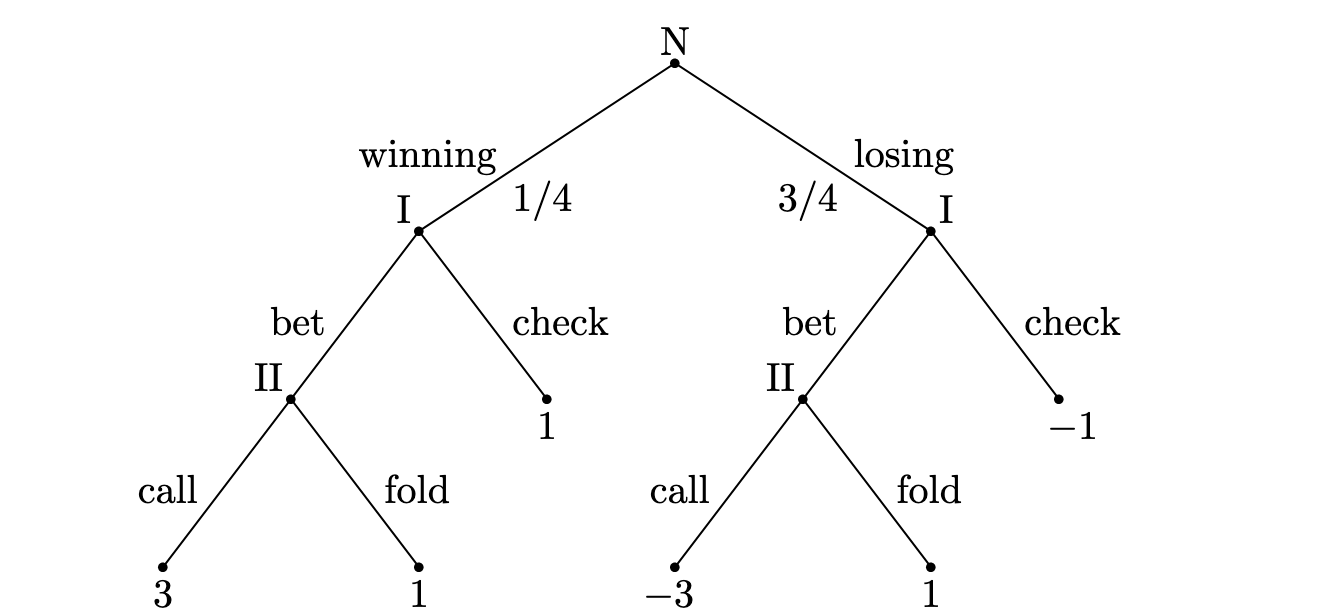
\includegraphics[width=0.8\textwidth]{Kuhn Tree.png}
    \caption{Game Tree}
\end{figure}

Depicted in figure 1, we have a game tree where there are at most three moves in this game: (1) the chance move that chooses a card for Alice, (2) Alice’s move in which she checks or bets, and (3) Bob’s move in which he folds or calls. To each vertex of the game tree, we attach a label indicating which player is to move from that position. Chance moves we generally refer to
as moves by nature and use the label $N$. 

Note, that Alice has two information sets. In each set (winning branch or losing branch) she must make a choice from among two options. Thus, yielding a total of four pure strategies:
\begin{itemize}
    \item $(b,b)$: bet with winning card or bet with losing card,
    \item $(b, c)$: bet with winning card, check with losing card,
    \item $(c, b)$: check with winning card, bet with losing card,
    \item $(c, c)$: check with winning card or check with losing card.
\end{itemize}
Figure 1 depicted the extensive form of a game. Formally that is the mathematical model of a game built on the basic notions of position and move given by a triplet $(X, Y, A)$, where
\begin{itemize}
    \item $X$ is a nonempty set, the set of strategies of Alice,
    \item $Y$ is a nonempty set, the set of strategies of Bob,
    \item $A$ is a real-valued function defined on $X \times Y$ . (Hence, A($x, y$) is a real number for every $x \in X$ and every $y \in Y$).
\end{itemize}

Thus, X = $\{(b, b), (b, c), (c, b), (c, c)\}$ and Y = $\{c, f\}$, where:
\begin{itemize}
    \item $c$: If Alice bets, call.
    \item $f$: If Alice bets, fold.
\end{itemize}

\textbf{Solve for A (payoff matrix):}

\[
    Alice (b, b), Bob (c): A((b, b), c) = \frac{1}{4}(3) + \frac{3}{4}(-3) = -\frac{3}{2}
\]
\[
    Alice (b, b), Bob (f): A((b, b), f) = \frac{1}{4}(1) + \frac{3}{4}(1) = 1
\]
\[
    Alice (b, c), Bob (c): A((b, c), c) = 0
\]
\[
    Alice (b, c), Bob (f): A((b, c), f) = -\frac{1}{2}
\]
\[
    Alice (c, b), Bob (c): A((c, b), c) = -2
\]
\[
    Alice (c, b), Bob (f): A((c, b), f) = 1
\]
\[
    Alice (c, c), Bob (c): A((c, c), c) = -\frac{1}{2}
\]
\[
    Alice (c, c), Bob (f): A((c, c), f) = -\frac{1}{2}
\]
\\
Thus, we obtaining given payoff matrix in Table 2.
\begin{table}[h]
    \centering
    \begin{tabular}{|l|c|c|}
        \hline
        & $c$ & $f$ \\ \hline
        $(b, b$) & -~3/2 & 1 \\ \hline
        $(b, c)$ & 0 & -~1/2 \\ \hline
        $(c, b)$ & -2 & 1 \\ \hline
        $(c, c)$ & -~1/2 & -~1/2 \\ \hline
    \end{tabular}
    \caption{Payoff Matrix A}
    \label{tab:payoff_matrix}
\end{table}
\\
Note that the third row is dominated by the first and that the fourth row is dominated by the second row, allowing us to simplify our payoff matrix to Table 3.
\begin{table}[h]
    \centering
    \begin{tabular}{|l|c|c|}
        \hline
        & $c$ & $f$ \\ \hline
        $(b, b)$ & -~3/2 & 1 \\ \hline
        $(b, c)$ & 0 & -~1/2 \\ \hline
    \end{tabular}
    \caption{Payoff Matrix A'}
    \label{tab:payoff_matrix}
\end{table}
\\
This too should make sense not only from a mathematical perspective, but also from a logic perspective as well. That is, it is very unlikely for Alice to play $(c, b)$ or $(c, c)$ as she would be checking a winning hand. Then we proceed by solving for the value of our game.
\\
\\
\textbf{Alice's expected winning if Bob plays $c$:}
\\
\[
    -\frac{3}{2}p + 0(1 - p) = -\frac{3}{2}p
\]
\textbf{Alice's expected winning if Bob plays $f$:}
\[
    1p + -\frac{1}{2}(1 - p) = 1p - \frac{1}{2} + \frac{1}{2}p
\]
\textbf{Equate Alice's expected winnings:}
\[
    1-\frac{3}{2}p = \frac{3}{2}p - \frac{1}{2}
\]
\[
    3p = \frac{3}{2}
\]
\[
    p = \frac{1}{2} \implies (1 - p) = \frac{1}{2}
\]
\\
We then calculate Bob's expected loss.
\\
\textbf{Bob's expected loss if Alice plays $(b, b)$:}
\[
    -\frac{3}{2}q + 1(1 - q) = -\frac{5}{2}q + 1
\]
\\
\textbf{Bob's expected loss if Alice plays $(b, c)$:}
\[
    0q + (-\frac{1}{2})(1 - q) = \frac{1}{2}q - \frac{1}{2}
\]
\textbf{Equate Bob's expected winnings:}
\[
    -\frac{5}{2}q + 1 = \frac{1}{2}q - \frac{1}{2}
\]
\[
    q = \frac{1}{2} \implies (1 - q) = \frac{1}{2}
\]
\\
\textbf{Value of game:} 
\\
Alas, we finally proceed by solving for the value of our game; that is, substituting $p$, $1 - p$, $q$, and $1 - q$ into our $2\times2$ payoff matrix and solving for the expected game value.
\[
    V = (-\frac{3}{2})(\frac{1}{2})(\frac{1}{2}) + (1)(\frac{1}{2})(\frac{1}{2}) + (0)(\frac{1}{2})(\frac{1}{2}) + (-\frac{1}{2})(\frac{1}{2})(\frac{1}{2}) = -\frac{1}{4}
\]
\\
Therefore, under optimal strategies: Alice can expect to lose $-\frac{1}{4}$ on average per game, while Bob gains $+\frac{1}{4}$ on average per game.

\section{Conclusion}

\hspace{\parindent} In this paper, we explored fundamental poker scenarios through simplified models to highlight optimal strategies in betting, bluffing, and calling situations. By analyzing toy games such as the clairvoyance, [0,1], AKQ, and poker endgames, we exhibited the underlying mathematical theories that guide optimal decision-making. Through concepts like bluff-to-bet ratios, equilibrium strategies, and the balance of risk versus reward, we illustrated how players can leverage probabilities and expected values to avoid exploitation and achieve optimal play. These games, while not representative of poker in its entirety, provide valuable insights into strategic thinking and the mathematical principles governing poker. Further work can generalize and advance these findings to incorporate additional complexities, coming closer to modeling a complete game of poker.

\section{Works cited}%we need mla style

[1] Chen, Bill, and Jerrod Ankenman. \textit{The Mathematics of Poker}. ConJelCo LLC, 2006. 
\newline
[2] Ferguson, Thomas S. \textit{A Course in Game Theory}. World Scientific Publishing Co. Pte. Ltd, 2023. 

\end{document}